\section{Materials and Methods}

\subsection{Experiments}
A total of 23 right-handed subjects took part in the experiment (9 females, 14 males, $24 \pm 4.6$ years old). All subjects were non-smokers and without respiration problems. According to their self-reports, none had a history of injury in the olfactory bulb or incapability of smelling. Subjects were informed about the experimental protocol and the purpose of the study. None of the participants in experiment were wearing perfumed products on the day of experiment. 

10 different odors were provided for the experiment, including rose water, lavender oil, jasmine oil, chocolate powder, mint oil, valerian pills, garlic powder, star anise, rotten cooked cauliflower and baby shampoo. The odorants were placed inside covered bottles so as to avoid effects of their visual characteristics.

After the set up of the EEG recording system, subjects were asked to relax and close their eyes. One odor bottle was randomly selected and provided to the subject's nostrils at 1-2 cm. The subjects were not informed about the name of the odor during the experiment. The same odor was presented for about 15 times, leading to about 15 trials. Each trial consisted of 6 seconds baseline and 6 seconds odor experience. After experiencing an odor, the subjects were asked to rate it in terms of pleasantness, using a 5-point Linkert scale that ranged from very unpleasant to very pleasant. 
%More details about the experiment can be found in~\cite{kroupi2014non}.     

Regarding the equipment, an EGI's Geodesic EEG system (GES) 300 was used to record, amplify and digitalize the EEG signals. EEG signals were recorded from a 256-channel EEG Net Amps 300 cap with sampling frequency of 250Hz.  

\subsection{Pre-processing of EEG Signals}
After the pre-cleaning and synchronization of recorded 256-channel EEG signals by GES-300 system, a total of 12 seconds EEG segment is kept for each trial. It contains 6 seconds of baseline (resting state) and 6 seconds of activity (odour perception). Signals from 40 electrodes which locate on face muscles and around eyes are rejected in order to reduce muscle and eye movement artifacts. Signals from the remaining 216 electrodes are kept for further analysis. 

A bandpass filter (4th order butterworth) is applied for the EEG signals with pass-band 0-50Hz. Small laplacian filter is applied for each electrode in order to reduce volume conduction effects~\cite{wolters2007volume}. Remaining Eye-movement artifacts are rejected manually by using Independent Component Analysis (funcitons are provided by EEGLAB\copyright~ toolbox~\cite{luck2014introduction}). Topographic maps of ICA components are plotted for each trial, components showing strong activities around eye-region are examined and rejected if their statistics confirms that they are artifact components~\cite{luck2014introduction}. The number of components removed varies for each trial of each subject. 

\subsection{Construction of Functional Connectivity Networks}
Functional connectivity can be estimated in various ways. Two time-doman functional connectivity models were applied and compared in this paper, which are Linear Granger Causality model~\cite{roebroeck2005mapping}  and Nonlinear Regression Analysis model~\cite{bettus2008enhanced}. We applied both models to our 216-channel EEG signals and the performances of estimated functional connectivity networks were analysed by the classification on pleasantness during olfactory perception. The details on how to estimate functional connectivity networks by using these two models are described below.

\subsubsection{Linear Granger Causality}
Granger causality is first proposed by C.W.J. Granger in investigating causal relations in econometric models in 1969~\cite{granger1969investigating}. Decades later this concept is introduced into various neurophysiological studies. It is used to measure the causality between activities in different neuron assemblies, which estimates the functional connectivity over brain regions. 

Suppose we have two time series $X_t$ and $Y_t$. Let $U_t$ denote all the information accumulated from both time series since time $t-1$, and $U_t-Y_t$ denotes all this information apart from the specified series $Y_t$. $\sigma^2(X|U)$ is the variance of $\epsilon_t(X|U)$, in which $\epsilon_t(X|U)=X_t-P_t(X|U)$ and $P_t(X|U)$ represents the optimal, unbiased, least-squares predictor of $X$ using the set of values $U$.

\emph{Definition of Causality}: If $\sigma^2(X|U)<\sigma^2(X|\overline{U-Y})$, then Y is causing X, denoted by $Y_t \Rightarrow X_t$. Under the notion of Granger causality, $Y_t$ is causing $X_t$ if $X_t$ is better predicted using all available information than if the information from $Y_t$ is excluded.

The time series $X_t$ and $Y_t$ are represented by the signals from 2 different channel signals in our 216-channel EEG signal recordings. In this paper we used the Vector Auto-Regression model (VAR)~\cite{barnett2014mvgc} to estimate Granger causality since it provides better computational efficiency and numerical accuracy~\cite{barnett2014mvgc}. We used the MVGC toolbox~\cite{barnett2014mvgc} to estimate the parameters in the VAR model and to compute Granger causality. Details on the computing of Granger causality can be refered to~\cite{barnett2014mvgc}.

For our 216-channel EEG signals for each experiment trial, the Granger causality of each channel combination are computed, thus formed a $216 \times 216$ Granger causality matrix. This matrix describes the functional connectivity patterns among these 216 channels of each ordor presentation trial. 

\subsubsection{Nonlinear Regression Analysis}
Nonlinear regression analysis is also a commonly used model to estimate the functional connectivity. This model is introduced by Pijin and Lopes Da Silva for EEG analysis~\cite{pijn1990localization}. Nonlinear regression analysis can quantify the relationships between different EEG signals in order to determine whether activity in one neuron assembly depends on that of other assemblies.


Suppose we have two channels of EEG signals $x$ and $y$, then nonlinear regression analysis measures the \emph{correlation ratio} between two signals $x$ and $y$. The \emph{correlation ratio} ($\eta^2$) describes the dependency of signal $y$ on signal $x$. Assume the amplitude of signal $y$ is a function of the amplitude of signal $x$. The expectation of $y$ given a value of $x$ is denoted as $\mu_{y|x}$ where:
\begin{equation} \label{eq:regressioncurve}
\mu_{y|x} = \int_{-\infty}^{\infty} y p(y|x) \mathrm{d}y,
\end{equation}
and $\mu_{y|x}$ describes the predicted value of $y$ given $x$. By this definition, we can calculate the correlation ratio ($\eta^2$) by predicting $y$ value using $\mu_{y|x}$. $\eta^2$ is expressed as:
\begin{equation} \label{eq:NRAregression}
\eta^2 = \frac{Explained \ Variance \ of \ y \ giving \ x }{Total \ Variance \ of \ y}
\end{equation}
Explained variance is the variance calculated from $y$ according to $\mu_{y|x}$. In this paper, the nonlinear regression analysis algorithm is implemented by fieldtrip toolbox\copyright~\cite{oostenveld2010fieldtrip}. 


Similarly to the functional connectivity network construction using Granger causality, the estimation of functional connectivity network using Nonlinear regression analysis is done for all the channel combinations in our 216-channel EEG signals. The functional connectivity network for each ordor presentation trial is also of size $216 \times 216$ .

\subsection{Significance Check}
The significance check is similar for both methods (Grancer causality and Nonlinear Regression Analysis) and is split into two main parts: (1) $p$-value calculation for samples based on theoretical asymptotic null distribution; (2) statistical significance adjusted for \emph{Bonferroni} correction. The rationale behind applying a significance check is to keep only the significant connections. 

The \emph{null hypothesis} $H_0$ is set to "there is no functional connectivity between two channels". In this paper, we assume that the connectivity values emanate from a normal distribution and the $p$-value that rejects the null hypothesis is set to $p=0.05$. The commonly used $F$-statistics is applied for estimating the $p$-value both for Granger Causality and for Nonlinear Regression Analysis.

All the values in functional connectivity maps that passed significance check are kept for feature extraction and classification in later steps. The significance check was run after the estimation of functional connectivity maps for each trial of each subject. Thus the number of values that passed significance check were different across all trials. 

%\begin{Fig.}[!t]
%    \centering
%    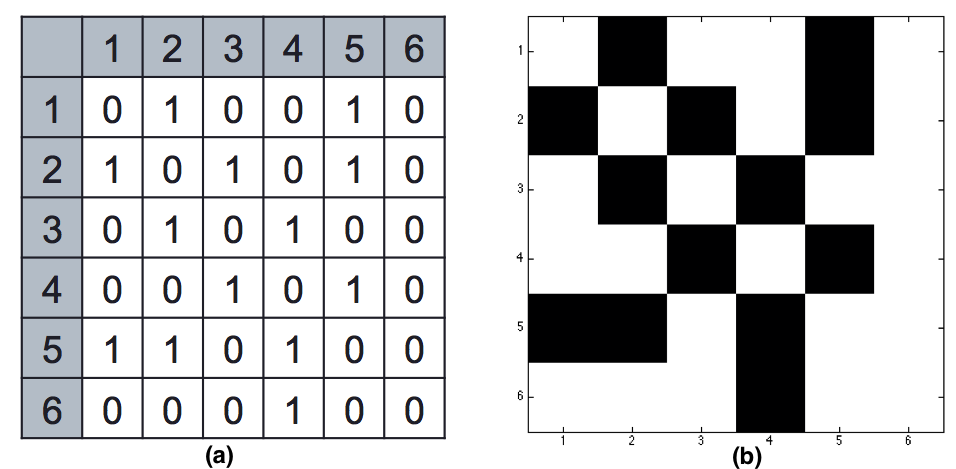
\includegraphics[width=0.45\textwidth]{./images/unweightednetwork.png}
%    \caption{An example of unweighted functional connectivity map construction of size $6 \times 6$. Nodes in (a) with value 1 represents the nodes that passed significance check. (b) is a visual expression of unweighted functional connectivity map.}
%    \label{fig:unweightednetwork}
%\end{Fig.}


%\begin{figure}[!t]
%    \centering
%    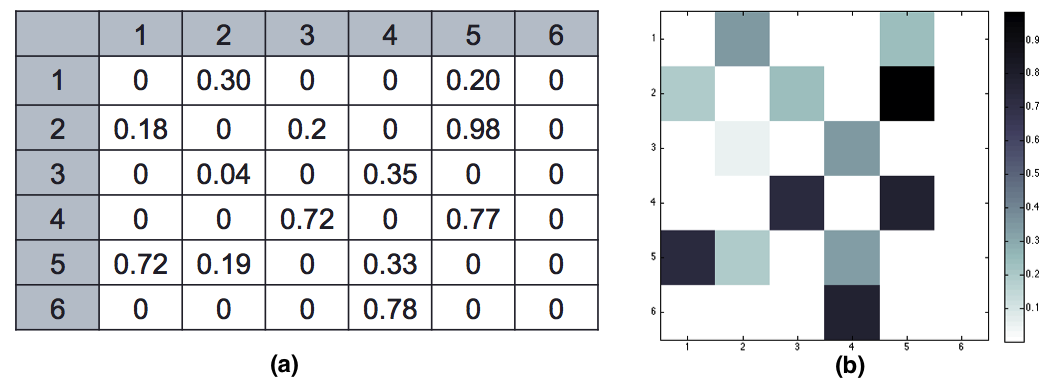
\includegraphics[width=0.45\textwidth]{./images/weightednetwork.png}
%    \caption{An example of a weighted functional connectivity map of size $6 \times 6$. In (a) the values represent the weights of the nodes. Each weight corresponds to the value of the underlying functional connectivity map. (b) A visual presentation of the same weighted functional connectivity map.}
%    \label{fig:weightednetwork}
%\end{figure}

\subsection{Network Feature Extraction}
As described in the Background section, it is difficult to analyse a functional connectivity network of size $216 \times 216$. The better way to evaluate such a large network is to extract useful features from it. Thus we introduced two types of network features to represent the functional connectivity networks. 

\subsubsection{Small-World Network Features}
The brain is considered as a small-world network by some group~\cite{bassett2006small}. Different aspects of small-world network has been studied and here, based on the commonly used features in neural network studies, we introduce four features for analysing our functional connectivity maps which are \emph{characteristic path}, \emph{global efficiency}, \emph{local efficiency} and \emph{clustering coefficient}~\cite{watts1998collective}~\cite{latora2001efficient}.

\emph{Characteristic path} represents the average shortest path of the network. The minimum value is achieved when the network is a complete graph (every pair of distinct vertices is connected by a unique edge). In our case, we can interpret the characteristic path as a feature representing the number of connections in the functional connectivity networks. The more the connections in the functional connectivity network, the smaller the value of the characteristic path, thus the faster the information that is transferred through the network. 

The concept of \emph{global efficiency} of a small-world network is introduced by Latora and Marchiori~\cite{latora2001efficient} and provides a measure of efficient behaviour of the network, by assuming that the network system is parallel (i.e., every vertex sends information concurrently through its edges in the network). The global efficiency of the network is higher when the characteristic path is short. Thus, global efficiency measures how efficiently the vertices exchange information through the network concurrently. Similarly with global efficiency, \emph{local efficiency} is defined as the average efficiency of the subgraphs of the neighbours of a vertex $i$ in the graph (details of computing subgraphs can be referred to~\cite{ullmann1976algorithm}). The subgraphs of $i$ do not contain vertex $i$, hence, the local efficiency can show how efficient the communication is when $i$ is removed from the network. Thus the local efficiency reveals how much the network is fault tolerant. 

Finally, \emph{clustering coefficient} of a network measures the degree to which vertices in a graph tend to cluster together. The overall level of clustering in a network is given by Watts and Strogatz~\cite{watts1998collective} as the average of the local clustering coefficients of all vertices. 

The mathmatical presentations and calculations of these 4 small-world network features can be refered to~\cite{rubinov2010complex}.

\subsubsection{Scale-Free Network Features}
A few studies have shown that brain functional connectivity can also be considered as a scale-free network. Groups of CJ Stam~\cite{stam2004functional} have found that brain functional connectivity network can be viewed as a scale-free network because the connectivity distribution followed a power-law scaling with an exponent close to two.
%, which suggests such functional connectivity network can be considered as a scale-free network topology~\cite{van2008small}. Detailed analysis can also be found in Thivierge's work~\cite{thivierge2014scale}.

In information theory, \emph{entropy} plays an important role in measuring uncertainty. Recently, following theoretical and statistical mechanics paradigms, several entropy measures for complexity have been proposed for network structures, and these measures have shown good performance in quantifying the level of organisation encoded in structural features of scale-free networks. It is well known that \emph{Shannon entropy} and \emph{von Neumann entropy} are related to the information present in classical and quantum systems respectively. Both of them can be used to analyse the structural organisation of scale-free networks\cite{anand2009entropy}. 

The amount of \emph{Shannon entropy} has a correlation with the number of network structural constraints. Examples of network constrains include: a) fixed number of links per vertex, b) given degree sequence (a monotonic non-increasing sequence of the degrees of vertices in the graph), and c) community structure (vertices of the network can be easily grouped into sets of vertices such that each set of vertices is densely connected internally). From this point of view, we can conclude that Shannon entropy has a clear interpretation of quantifying the information presented in network structure (Detailed proof can be referred to~\cite{anand2009entropy}). If a network has a smaller Shannon entropy, it will have more constrains on its structure, which shows this network is more optimal. 

\emph{Von Neumann entropy} has been defined by von Neumann for proving the irreversibility of quantum measurement processes. Recently it is also shown that von Neumann entropy can also be applied to network analysis~\cite{passerini2008neumann}. It has been shown that von Neumann entropy is a measure of regularity of networks~\cite{passerini2008neumann}. For a fixed number of edges, regular networks (networks whose vertices have the same number of neighbours) have in general a higher von Neumann entropy. It is also shown that von Neumann entropy depends on the number of connected components, long paths and nontrivial symmetries. With a fixed number of edges, von Neumann entropy is smaller for networks with higher degree of cluster. The mathematical proofs can be found in~\cite{passerini2008neumann} and~\cite{anand2009entropy}.

The mathmatical presentations and calculations for Shannon entropy can be refered to~\cite{lin1991divergence}, while the presentations and calculations for von Neumann entropy can be referred to~\cite{passerini2008neumann}.

Thus, to sum up, we provided two types of network features to measure the characteristics of our functional connectivity networks from different aspects of view. These networkfeatures including characteristic path, local efficiency, global efficiency, clustering coefficient, Shannon entropy and von Neumann entropy were extracted from the estimated functional connectivity networks for classification purposes. In particular, network features of Linear Granger Causality estimated functional connectivity networks and network features of Nonlinear Regression Analysis estimated functional connectivity networks were extracted separately for classification. We compared these two functional connectivity models by evaluating the classifiers' performances. 

\subsection{Classification}
Network features of previously estimated functional connectivity networks were extracted for both pleasant and unpleasant trials. For the purpose of classification, pleasant trials were labelled as 1 while unpleasant trials were labelled as 0. The whole dataset containing extracted features of 23 subjects is split into three parts. Feature data of 1 subjects formed the testing set, the left feature data of 22 subjects were further split into two subsets: training set and validation set. Validation set was used for selecting the best parameter of the classifier. Of the 22 subjects data, each time 1 subject was picked out and used as validation set while the others were used as training set (leave-one-subject-out cross-validation strategy). The parameter validation process was run for 22 times until all 22 subjects data were used for validation. The best parameter was selected based on which parameter value gave the best performence acrossing 22 validations.    

Support vector machine with a \emph{Gaussian radial basis function} kernel is used for classification. We tested 13 different values of parameter $\sigma$ ranged from 0.01 to 2 with regular space of 0.15. This range was selected based on try and trials. We tried the parameters ranged from 0.01 to 10 and found the best parameters always fell into the range of 0.01 to 2. Cohen's kappa $\kappa$~\cite{uebersax1987diversity}, as a measure of agreement between two viewers, and was used to evaluate the classifier's performance. Cohen's kappa is considered an accurate metric for classification performance and takes into account unbalanced classes (i.e., classes with different number of samples). 

Since we had data from 23 subjects and each time we used 1 of them for testing the performance of the classifier, to evaluate the overall performance of the classifier, the classification process was run for 23 times. Each time 1 subject's data was selected as testing set, while the others for training and parameter validation. After 23 times, all 23 subjects' data were used for testing the classifier and the evaluation was based on the 23 resulting Cohen's kappa values. 
